\chapter{プロセスとジョブ}

%==============================================================================
\section{プロセス}
皆さんは,これまでPCを使用してきた経験から,
\figref{pc}に示すように,
同時に複数のプログラムがPCで実行されていることを理解しているだろう.
また,同じプログラムが複数のウインドで同時に実行されることがある
ことも理解しているだろう\footnote{
\figref{pc}の例では二つのターミナル(Terminal)夫々の中で,
合計二つのa.outが同時に実行されている.
}.

つまり,一連の機械語命令である\emph{プログラム}だけでなく,
実行中のプログラムのインスタンスも意識する必要がある.
実行中のプログラムのインスタンスのことを\emph{プロセス}と呼ぶ.

\begin{center}
  \emph{\Large プロセス = 実行中のプログラム}
\end{center}

\begin{myfig}{btp}{PC上の複数プログラム}{pc}
  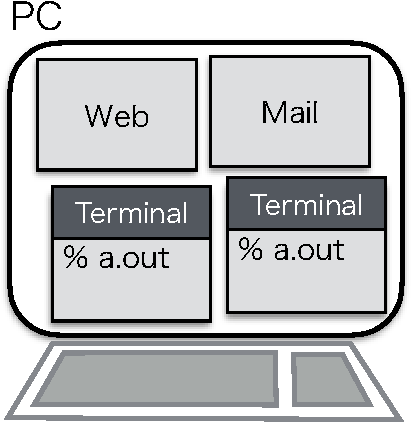
\includegraphics[scale=0.7]{Fig/pc-crop.pdf}
\end{myfig}

\subsection{プロセスの構造}

\figref{proc}にプロセスの構造を模式的に示す.
プロセスは,
プロセス名(プロセス番号)等の「プロセスの情報」や,
前回プロセスを実行中だった時の「CPUの状態」を保存する領域(仮想CPU)と
そのプロセス専用の「メモリ空間」(仮想メモリ)を持つ.
一つ一つのプロセスが一台のコンピュータに相当するるものを備えており,
プロセスを一台の\emph{仮想コンピュータ}と考えることもできる.

\begin{center}
\emph{\Large プロセス = 仮想コンピュータ}
\end{center}


\begin{myfig}{btp}{プロセスの構造}{proc}
  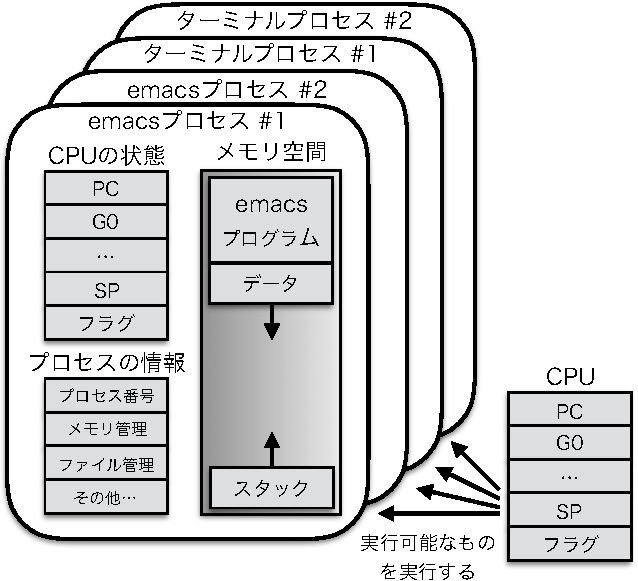
\includegraphics[scale=0.7]{Fig/proc-crop.pdf}
\end{myfig}

PC内には多数のプロセスが同時に存在し,
これらの中から実行可能なもの\footnote{
例えば,ユーザのキー操作待ちのものは実行不可能なプロセスである.}
を一つ\footnote{CPU(コア)が複数ある場合は一つとは限らない.}
選択し実物のCPU(実CPU)で実行する.
実行するプロセスを短時間に次々切替えることにより,
複数のプロセスが同時に実行されているように見せかけることもできる.

\subsection{プロセス関連のUNIXコマンド}

\subsubsection{psコマンド}
PC内で実行中のプロセスの一覧表を状態付きで表示するコマンドである.
macOSでターミナルを二つ開いた状態で,
一方のターミナルでvi(vim)を起動し,
もう一方のターミナルでpsコマンドを実行した例をリスト\ref{ps1}に示す.

\lstinputlisting[numbers=none,
  caption=psの実行例,float=btp,label=ps1]{Lst/ps.txt}

全てのプログラムはプロセスとして実行される.
ターミナルやpsコマンド自身もプロセスとして実行されるが,
macOSの標準では,これらは表示されない.
\texttt{-zsh} はターミナルに入力されたコマンドを解釈して実行するシェルである.
表示内容の意味は\tabref{psOut}\footnote{
リスト\ref{ps1}の実行例に含まれていない項目も含んでいる.}の通りである.

制御端末はプロセスがどのターミナルで実行されているかを示す.
ターミナルの名前はリスト\ref{ps1}の最後の部分のように,
ターミナルでtty コマンドを実行すると確認できる.

%\lstinputlisting[numbers=none,float=btp]{Lst/tty.txt}

\begin{mytable}{btp}{psコマンドの表示内容}{psOut}
  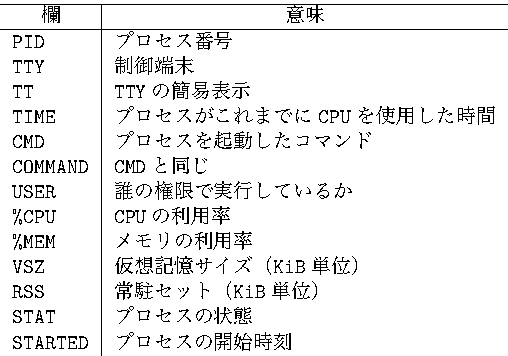
\includegraphics[scale=1.0]{Tbl/psOut.pdf}
\end{mytable}

\subsubsection{psコマンドのオプション}
\tabref{psOptions}にpsコマンドのオプションの一部を
\footnote{
最近のUNIXではpsコマンドのオプションが大きく変更されている.
詳しくは,各自で\texttt{man 1 ps}を用いて調べること.
なお,macOSのpsでは古いオプションも使用できるので,
ここでは簡単で分かりやすい古いオプションの使用例を示す.
}
リスト\ref{ps2}にオプションを用いた時の実行例を示す.
\texttt{ps u}を実行するとリスト\ref{ps1}と同じ三つのプロセスに付いて,
より詳しい表示がされた.
表示内容の意味は\tabref{psOut}の通りである.
プロセスの状態は,\tabref{psStat}の二文字を組合せて表現される.
例えば,リスト\ref{ps2}で\texttt{vi}は\texttt{S+}なので,
フォアグラウンドで実行中に短期間のスリープをしていることが分かる.

\begin{mytable}{btp}{psコマンドのオプション(一部)}{psOptions}
  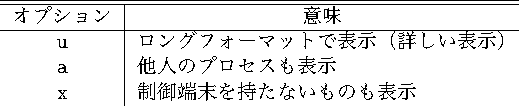
\includegraphics[scale=1.0]{Tbl/psOptions.pdf}
\end{mytable}

\lstinputlisting[numbers=none,caption=psコマンドのオプション付き実行例,
  float=btp,label=ps2]{Lst/psLong.txt}

\begin{mytable}{btp}{psコマンド\texttt{STAT}表示の意}{psStat}
  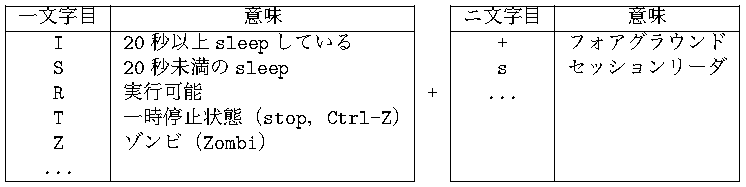
\includegraphics[scale=1.0]{Tbl/psStat.pdf}
\end{mytable}

\texttt{ps au}を実行すると\texttt{root}\footnote{
UNIX系のオペレーティングシステムでは,
システム管理者の名前が\texttt{root}である.}のプロセスも表示されている.
\texttt{u}オプションも付けているので詳しい表示形式になっている.
この実行例では ps コマンド自身も表示されている.
ps コマンドは\texttt{root}のプロセスとして実行されていたことが分かる.

\texttt{ps aux}を実行すると全ユーザの全プロセスが表示される.
\texttt{TT}が「\texttt{??}」のプロセスが制御端末を持たないものである.
macOSでは色々な権限で600程度のプロセスが実行されていることが分かる.

\subsubsection{killコマンド}

プロセスにシグナル(ソフトウェア割込み)を送るコマンドである.
通常,プロセスは予期しないシグナルを受取ると終了する.
killコマンドはシグナル(省略可能)とプロセス番号を引数にする.
使用できるシグナルの一部を\tabref{kill}に,
使用例をリスト\ref{sleepKill}に示す\footnote{
コマンド行から簡単に起動できて,しばらく実行し続ける sleep を例にする.
}.

\begin{mytable}{btp}{\texttt{kill}コマンドのシグナル名と番号(一部)}{kill}
  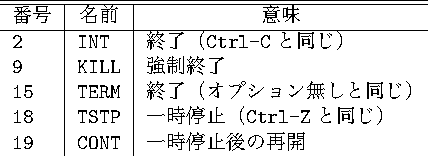
\includegraphics[scale=1.0]{Tbl/killOptions.pdf}
\end{mytable}

\lstinputlisting[numbers=left,caption=killコマンドの使用例,
  float=btp,label=sleepKill]{Lst/kill.txt}

\begin{description}
\item[1行] sleep をバックグラウンドで起動する.
\item[2行] sleep はジョブ番号1,プロセス番号75868で起動した.
\item[3行] ps コマンドで確認してみる.
\item[7行] sleep にTERMシグナルを送信してみる.(シグナル名は省略)
\item[8行] sleep は終了した.
\item[9行] sleep を再度バックグラウンドで起動する.
\item[11行] sleep にTSTPシグナルを送信してみる.
\item[12行] sleep は一時停止した.
\item[13行] sleep が存在し続けていることを確認する.
\item[17行] sleep にCONTシグナルを送信してみる.(動き始めたはず)
\item[18行] シグナル名を省略したのでTERMシグナルが送られたはず.
\item[19行] sleep は終了した.
\end{description}

%==============================================================================
\section{ジョブ}
ジョブはユーザの視点からはプロセスとよく似たものに見える.
ジョブはシェルが管理するプロセスのグループである.
シェルは一度に起動されたひとまとまりのプロセスを一つのジョブとして扱う.
リスト\ref{job}に例を示す.

\lstinputlisting[numbers=none,caption=ジョブの例,label=job,float=btp]
                {Lst/job.txt}

\subsection{ジョブの種類}
ジョブにはフォアグラウンド・ジョブとバックグラウンド・ジョブの2種類がある.
夫々、次のような特徴がある.実行例はリスト\ref{fgbg}の通りである.

\begin{description}
\item[フォアグラウンド・ジョブ]
シェルがジョブの終了を待つ.
ジョブが終了したらプロンプトが表示される.

\item[バックグラウンド・ジョブ]
コマンドの最後に\texttt{\&}を付けて実行する.
シェルがジョブの終了を待たない.
ジョブが終了していなくてもプロンプトが表示される.
次のジョブと並列実行ができる.
\end{description}

\lstinputlisting[numbers=none,caption=フォアグラウンド・バックグラウンド,
    float=btp,label=fgbg]{Lst/fgbg.txt}

\subsection{ジョブ制御}
シェルと制御端末はジョブに対して働きかけをすることができる.

\begin{description}
\item[Ctrl-C] フォアグラウンド・ジョブにINTシグナルを送る.
(通常,ジョブは終了する.)

\item[Ctrl-Z] フォアグラウンド・ジョブにTSTPシグナルを送る.
(ジョブは一時停止状態になる.)

\item[jobs] そのシェルが管理しているジョブの一覧を表示する.

\item[fg] バックグラウンド・ジョブや一時停止中のジョブを
フォアグラウンドに切替える.
ジョブ番号を指定することもできる.

\item[bg] 一時停止状態のジョブをバックグラウンドで再開する.
ジョブ番号を指定することもできる.
\end{description}

リスト\ref{jobControl}にジョブ制御の使用例を示す.

\lstinputlisting[numbers=left,caption=ジョブ制御の使用例,
  float=btp,label=jobControl]{Lst/jobControl.txt}

\begin{description}
\item [1行] sleep をフォアグラウンドで起動する.
\item [2行] Ctrl-Z で sleep へTSTPシグナルを送る.(sleepは一時停止状態になる)
\item [4行] sleep をバックグラウンドで再開する.
\item [6行] もう一つの sleep をバックグラウンドで起動する.
\item [8行] 二つの sleep ジョブがあることを確認する.
\item [10行] ジョブ 2 がカレントジョブ
(ジョブを明示しないときの操作対象)である.
\item [11行] 番号を明示してジョブ 1 をフォアグラウンドに変更する.
\item [13行] Ctrl-C でジョブ 1 へINTシグナルを送る.(sleepは終了する)
\item [14行] sleep ジョブが一つだけになっていることを確認する.
\end{description}

%==============================================================================
\section*{課題 No.5}
\begin{enumerate}
\item 本文と照らし合わせながらプロセスの
実行例(リスト\ref{jobControl}まで)を試し,内容をよく理解しなさい.
一時停止状態のsleepを操作するとどうなるか等,よく観察すること.

\item 以下の操作方法を考えて手順を説明しなさい.

\begin{enumerate}
\item ターミナルが一つしか使用できない条件下で,
フォアグラウンドで暴走してしまった(Ctrl-Cで終了しなくなった)
ジョブを強制終了する手順.
(KILLシグナルを使用すること)

\item 間違ってフォアグラウンドで起動したsleepを
バックグラウンドに変更する手順.

\item バックグラウンドで実行中のジョブを
フォアグラウンドに変更してCtrl-Cで終了する手順.
\end{enumerate}

\end{enumerate}
